\chapter{Introduction}

\section{Motivation}
\subsection{Dataset size considerations}
\label{size_considerations}
From the very beginning it was clear that the size of the gathered data would be a problem to face carefully. To provide context, let us calculate how many bytes it would take to just store the world positions of the bounces of all paths needed to produce image \ref{hall_render}. It is 512 pixels wide and 512 pixels tall, it has been rendered with 512 samples per pixel --- spp --- each with a depth of maximum 10 --- this means that each of the 512 paths shoot every pixel bounced in the scene at most 10 times. Assuming every bounce position is stored as a triplet of single precision float numbers we would have:
\begin{equation}
	\label{rough_bounce_size_estimation}
	(512 \times 512) pixels \times 512 spp \times 10 bounces \times 3 dimensions \times 4 bytes \approx 15GB
\end{equation}
\begin{figure}
	\centering
	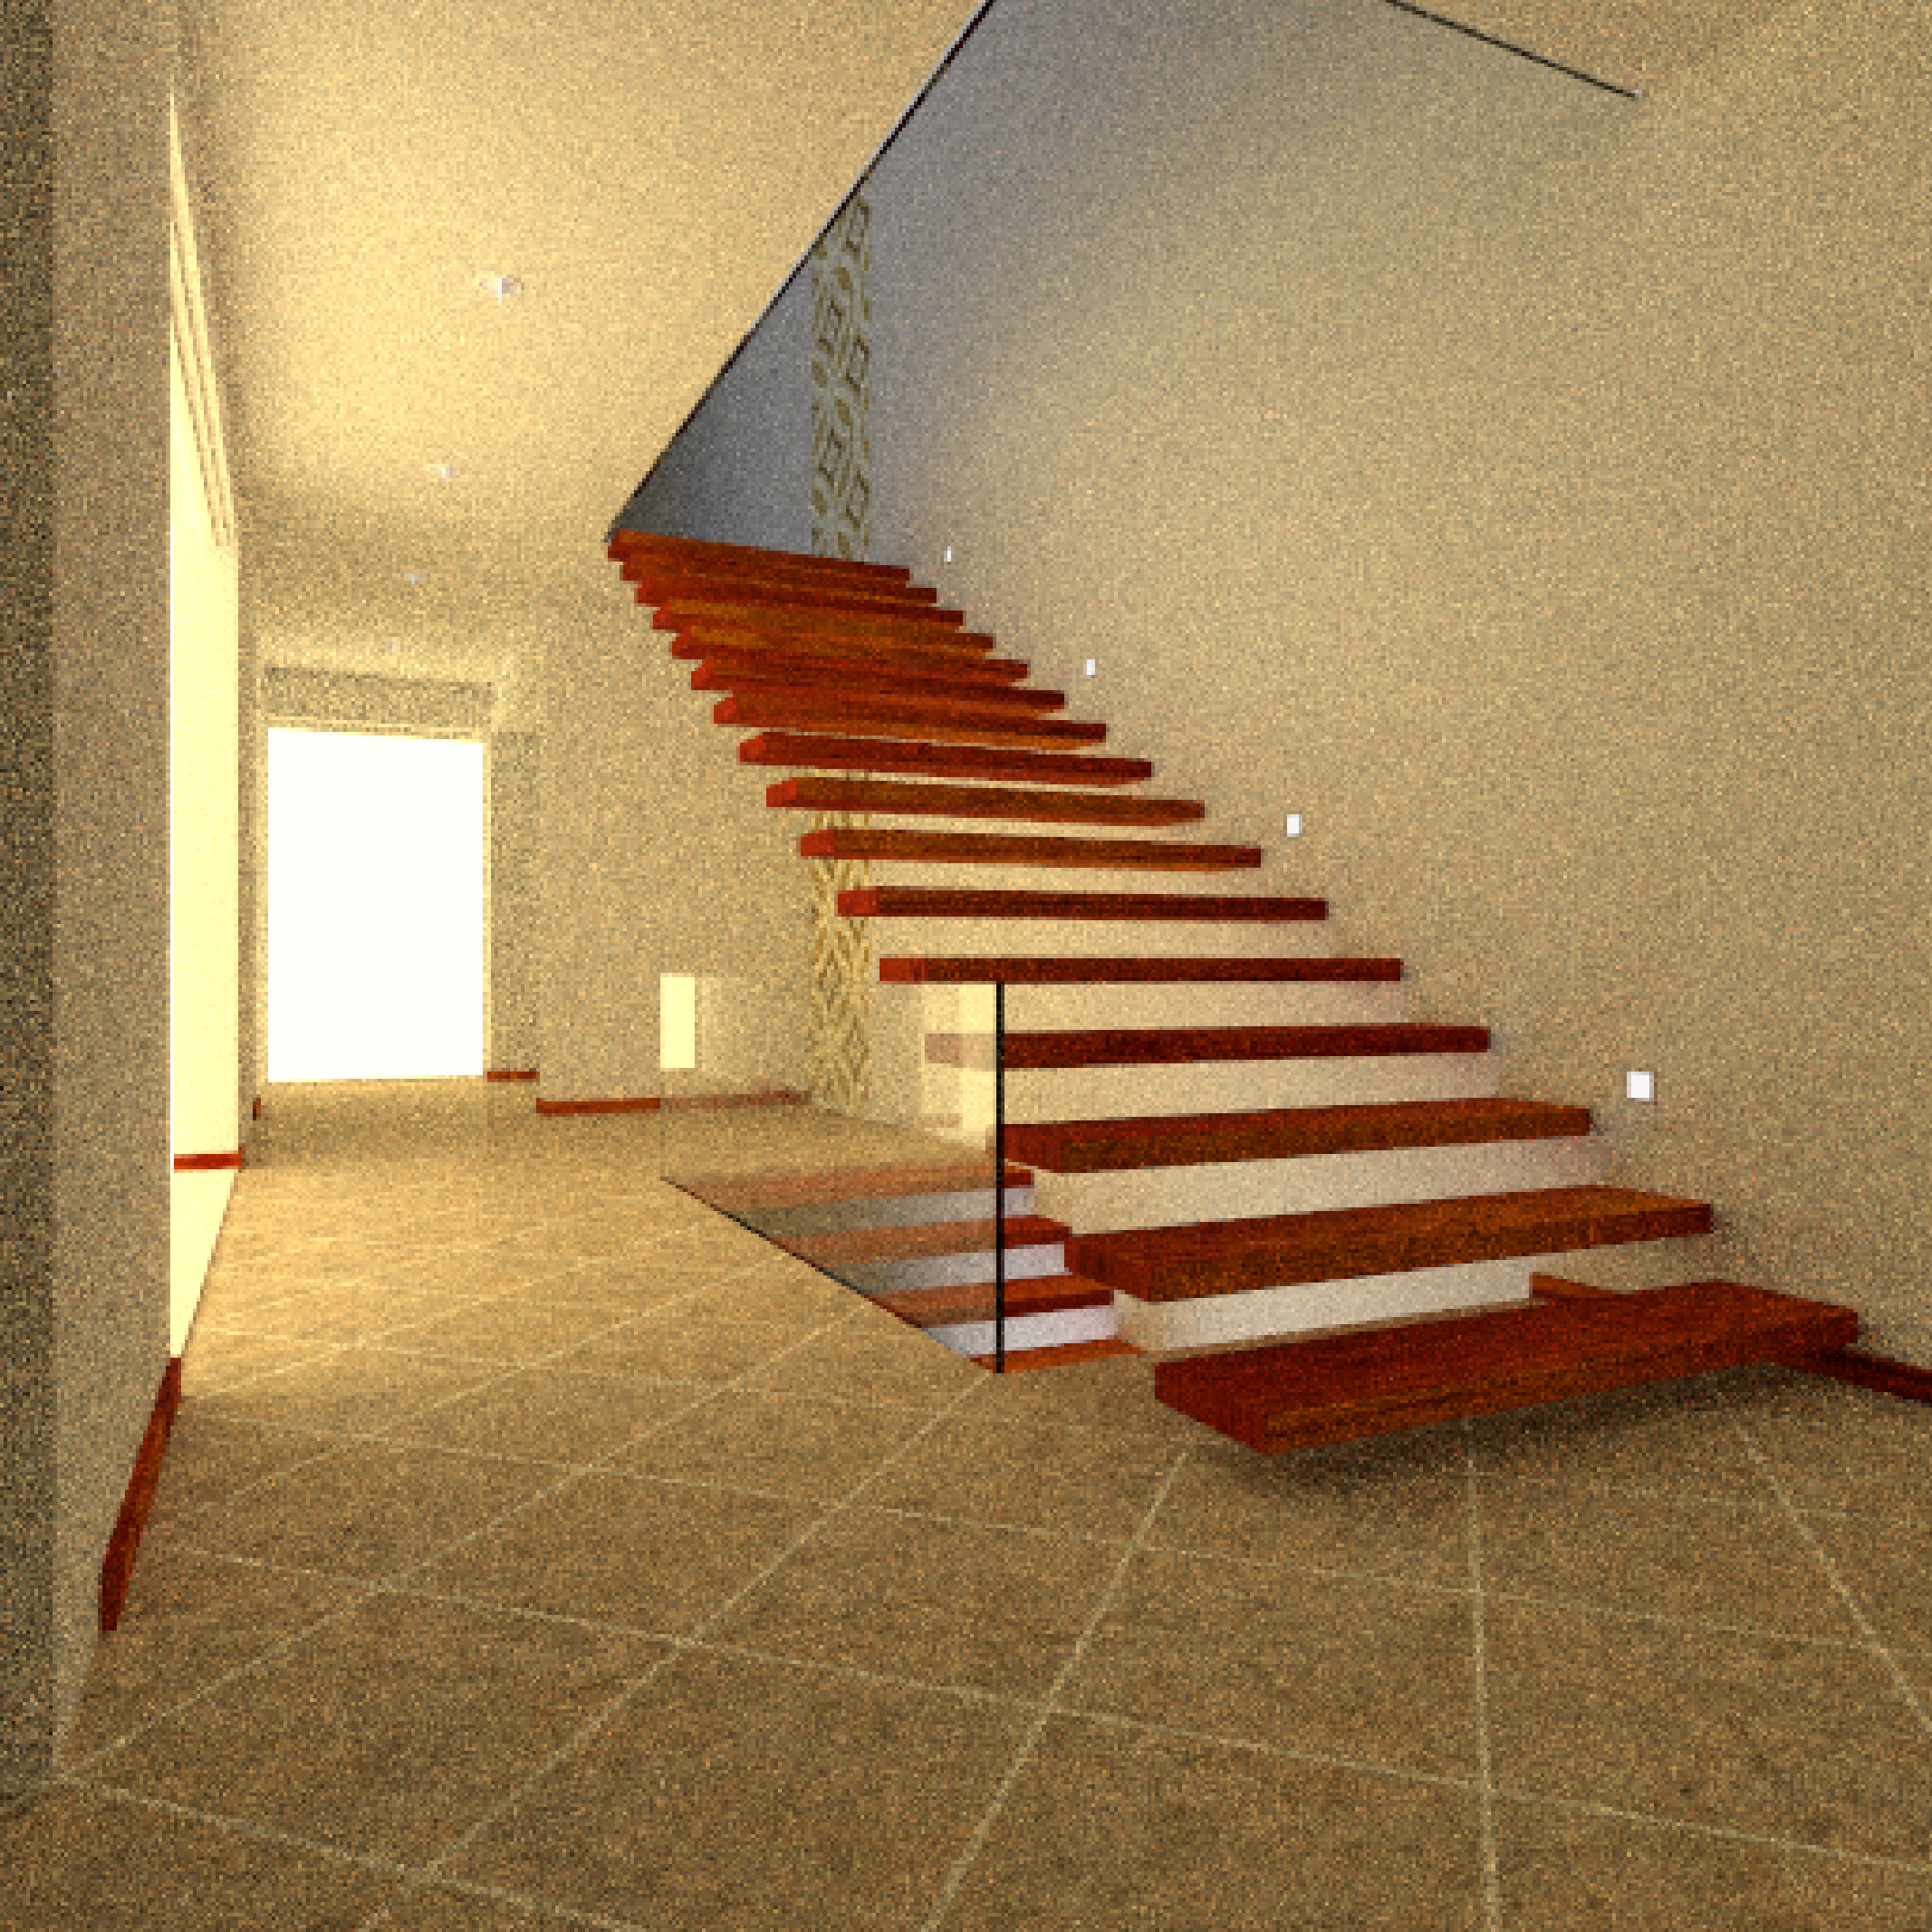
\includegraphics[height=8cm]{chapters/chapter_thetool/hall}
	\caption{\textit{Modern Hall} scene \cite{bitterliscenes} rendered by Yocto/GL \cite{pellacini2019yocto}. It is a 512x512, 512spp image; maximum bounces per path are set to 10.}
	\label{hall_render}
\end{figure}
It has been assumed that every path bounces exactly 10 times before being terminated, but in reality most paths are terminated way before either when they bounce out of the scene or --- in some path tracers --- they hit a light. This leads to a reduction of the 15GB shown in equation \ref{rough_bounce_size_estimation} but also to the need of an additional buffer storing the amount of bounces each path has. This new buffer needs to contain integers and, considering that the standard \texttt{int} type on x86\_64 machines is 4 bytes long, we would have that its size --- still in the figure \ref{hall_render} context --- would approximately be:
\begin{equation}
	\label{rough_lenghts_size_estimation}
	(512 \times 512) pixels \times 512 spp \times 4 bytes \approx 500MB
\end{equation}
Now this is not an unmanageable amount of data, but since the tool had to be usable on consumer grade machines, reducing those number has been one of the main priorities during the early stages of development. The most effective change that has been made was to simply use smaller primitive data types. 

Single precision floats had been almost immediately replaced with half-precision floating point numbers, effectively halving the size of the world positions buffers. Using the same assumptions made for equation \ref{rough_bounce_size_estimation}, we would have 7.5GB instead of 15GB.
Halving precision, beside a memory footprint reduction, comes with a reduction of actual precision and potential noticeable rounding errors; but since these numbers will mostly be directly used for visualization purposes with very little processing, errors should not negatively impact the user experience. C++ does not have a built-in \texttt{half} type so an IEEE 754 compatible header only library\footnote{\url{http://half.sourceforge.net/}} has been used thoroughly the written software.

Considering now the paths lengths buffer, in most reasonable cases, 1 byte per path would suffice: 255 bounces are more than enough for most cases. Examining equation \ref{rough_lenghts_size_estimation}, after the reduction from 4 bytes to 1 that buffer occupies approximately 128MB.